%\newcommand{\F}{\mathbb{F}}
%\newcommand{\G}{\mathbb{G}}
\newcommand{\Cdel}{\ensuremath{c_{del}}}
\newcommand{\Cins}{\ensuremath{c_{ins}}}
\newcommand{\Cupd}{\ensuremath{c_{upd}}}
\renewcommand{\O}[1]{\ensuremath{\mathcal{O}(#1)}}

%indentation in code:
\algdef{SE}[SUBALG]{Indent}{EndIndent}{}{\algorithmicend\ }
\algtext*{Indent}
\algtext*{EndIndent}


\chapter{Tree-edit-distance algoritmus}

Jadro aplikacie lezi v pouziti tree-edit-distance (TED) algoritmu,
vdaka ktoremu dostaneme mapovanie medzi 2 RNA stromami. Mapovanie nam ukaze
spolocne casti oboch RNA stromov. TED algoritmus je obdoba Levenstheinoveho
string-edit-distance algoritmu. Problem u retazcov je specialnym pripadom
TED-u, kedy stromy zdegenerovali na cesty (spojovy zoznam).

\section{Hlavna myslienka TED-u}

Zaklad TED algoritmu je v rekurzivnom vzorci \ref{eq:ted} z \citet{DMRW} a \citet{RTED}. Vzdialenost medzi
lesmi F a G, $\delta(F, G)$ je definovana ako minimalny pocet editacnych operacii,
ktore z F urobia G. Pouzivame standardne editacne operacie - delete, insert, update.

\begin{figure}[H]
\centering
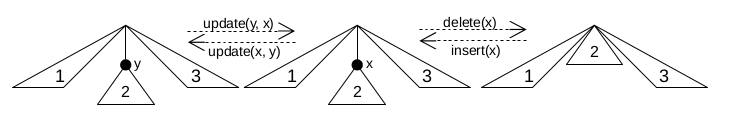
\includegraphics[width=140mm, height=30mm]{../img/TED_operations.png}
\caption{Ukazky TED operacii}
\label{obr:TED_operations}
\end{figure}

Delete, zmazanie vrcholu, znamena pripojit k predkovi vsetkych jeho potomkov so
zachovanim poradia medzi nimi. Insert, vlozenie vrcholu, je opacna operacia k
delete, co znamena, ze vkladame vrchol medzi rodica nejakych jeho, po sebe
nasledujucich potomkov. Update iba zmeni hodnotu vo vrchole stromu.

\section{Znacenie}

V tejto kapitole sa budeme riadit znacenim \citet{RTED}. Teda, pouzivame definiciu
stromu a lesa z \ref{def:strom}. Ak $F$ je les (strom), $N_F$ oznacuje mnozinu jeho vrcholov a $E_F$
mnozinu jeho hran. Plati dalej ze $E_F \subseteq N_F \times N_F$. $\emptyset$ oznacuje
prazdny strom, resp. prazdny les. Podles lesa $F$ je graf $\tilde{F}$ s vrcholmi
$N_{\tilde{F}} \subseteq N_F$ a hranami $E_{\tilde{F}} \subseteq E_F \cap N_{\tilde{F}} \times N_{\tilde{F}}$.
Obdobne to plati aj pre podstrom stromu $T$.
$F_{v}$ oznacuje podstrom $F$ zakoreneny vo $v$, t.j. v strome ostavaju iba potomkovia $v$.
$F - v$ budeme znacit les, ktory dostaneme zmazanim vrcholu $v$ z $F$, spolu so vsetkymi hranami
zasahujucimi do $v$. Podobne $F - F_{v}$ budeme znacit les, ktory dostaneme zmazanim podstromu
$F_{v}$ z $F$.

\begin{definice}[Editacna vzdialenost]
	Nech F a G su dva lesy. Editacna vzdialenost, tree-edit-distance - $\delta(F, G)$,
	medzi F a G je rovna minimalnej cene, za ktoru les F transformujeme na G.
\end{definice}

Vo vzorci \ref{eq:ted} pocitame editacnu vzdialenost $\delta(F, G)$,
\Cdel, \Cins a \Cupd su ceny zmazania, vlozenia a editacie vrcholu v strome
a $r_{F}$ a $r_{G}$ su korene, bud obidva najpravejsie alebo najlavejsie (tzn. vyberieme
najpravejsi/najlavejsi strom lesa a jeho koren).

\begin{figure}[H]\label{eq:ted}
\begin{subequations}
\begin{align}
	\begin{split}
	\delta(\emptyset, \emptyset) &=
		0
		\\
	\delta(F, \emptyset) &=
		\delta(F - r_{F}, \emptyset) + \Cdel(r_{F})
		\\
	\delta(\emptyset, G) &=
		\delta(\emptyset, G - r_{G}) + \Cins(r_{G})
	\end{split}
	\\[1ex]
	\delta(F, G) &=
		\begin{cases}
			\delta(F - r_{F}, G) + \Cdel(r_{F}) \\
			\delta(F, G - r_{G}) + \Cins(r_{G}) \\
			\delta(F - F_{r_{F}}, G - G_{r_{G}}) + \\
				\quad \delta(F_{r_{F}} - r_{F}, G_{r_{G}} - r_{G}) + \Cupd(r_{F}, r_{G})
		\end{cases}
\end{align}
\end{subequations}
\caption{Rekurzivny vzorec pre vypocet tree-edit-distance}
\end{figure}


\section{Algoritmy dynamickeho programovania}

\citet{TAI} predstavil algoritmus s priestorovou a casovou zlozitostou \O{m^3 \cdot n^3},
\citet{ZHANGSHASHA} algoritmus nasledne vylepsili pozorovanim toho, ze nepotrebujeme
vzdialenosti medzi vsetkymi parmi podlesov. Algoritmus mal casovu zlozitost \O{m^2 \cdot n^2}
a priestorovu \O{m \cdot n}. \citet{KLEIN} dosiahol casovu zlozitost \O{m^2 \cdot n \cdot \log{n}},
avsak jeho riesenie potrebovalo rovnako vela pamete.
\citet{DALUCQ} ukazali, ze minimalny cas na beh algoritmu je \O{m \cdot n \cdot \log{m} \cdot \log{n}}.
\citet{DMRW} predviedli worst-case optimalny algoritmus pre tree-edit-distance.
Jeho casova a priestorova zlozitost je \O{m^2 \cdot n \cdot (1 + \log{\frac{n}{m}})} a
\O{m \cdot n}. \citet{RTED} ukazali spojitost medzi efektivnostou predchadzajucich algoritmov
a tvarom stromov. Zovseobecnili predchadzajuce pristupy a vytvorili algoritmus beziaci
vo worst-case case \O{m^3} a priestore \O{m \cdot n}. Ich algoritmus je teda efektivny pre vsetky
tvary stromov a nikdy nespadne do worst-case, ak existuje lepsi smer vypoctu. 



\subsection{RTED: Robust Tree Edit Distance algoritmus}

Dalej sa v nasej praci budeme venovat vyhradne algoritmu RTED od tvorcov \citet{RTED}.
Ich algoritmus rozdelime na 2 casti, rovnako pomenovany RTED a GTED.

RTED (Robust Tree Edit Distance) algoritmus bude pre nas algoritmus na vypocet
optimalnej dekompozicnej strategie (viz definicia \ref{def:strategy})
a GTED (General Tree Edit Distance) algoritmus samotny vypocet rekurzie \ref{eq:ted}
s aplikovanim danej strategie.

\begin{definice}[Dekompozicna strategia]\label{def:strategy}
	Nech $F$ a $G$ su lesy. Dekompozicina strategia v rekurzii \ref{eq:ted} priradi
  kazdej dvojici podstromov $F_{v}$ a $G_{w}$ lesov $F$ a $G$ jednu cestu $\gamma_{T}$
  z korena do listu, kde $T \in \{F, G\}$.
	LRH dekompozicna strategia vybera vzdy najlavejsi/najpravejsi/najtazsi
	(left/right/heavy) vrchol na ceste z korena do listu. Najtazsi vrchol je taky
	v ktoreho podstrome je najviac vrcholov. 
\end{definice}


Zacneme principom fungovania GTED algoritmu. Detaily pre LRH strategie su
v \citet{ZHANGSHASHA} pre left/right a v \citet{DMRW} pre heavy strategiu.

\begin{algorithm}
  \caption{General Tree Edit Distance for LRH strategies}
  \label{alg:gted}
  \begin{algorithmic}[1]
    \Procedure {gted}{$F, G, TreeDistance, S$}
      \State $\sigma \gets S[F, G]$
      \If {$\sigma \in \sigma^{*}(F)$}
        \ForAll {$F' \in F - \sigma$}
          \State $TreeDistance \gets TreeDistance \cup \Call{gted}{F', G, TreeDistance, S}$
        \EndFor
        \State $TreeDistance \gets TreeDistance \cup \Call{$\Delta$}{F, G, TreeDistance, \sigma}$
      \Else
        \State $TreeDistance \gets TreeDistance \cup (\Call{gted}{G, F, TreeDistance^{T}, S^{T}})^{T}$
      \EndIf
      \State \Return{$TreeDistance$}
    \EndProcedure
  \end{algorithmic}
\end{algorithm}

\begin{algorithm}
  \caption{Single path function - part I}
  \label{alg:spf}
  \begin{algorithmic}[1]
    \Procedure {$\Delta$}{$F, G, TreeDistance, \sigma$}
      \State $ForestDistance \gets$ empty array $|F| + 1 \times |G| + 1$
      \label{alg:spf:init}
      \State $ForestDistance[\emptyset][\emptyset] := 0$
      \For {$F'$ subforest in \Call{get ordered subforests}{$F, \sigma$}}
        \State $Last_{F} \gets$ last added node to $F'$
        \State $ForestDistance[F'][\emptyset] := ForestDistance[F' - Last_{F}][\emptyset] +$
        \Indent
          \State $C_{del}(Last_{F})$
        \EndIndent
      \EndFor
      \For {$G'$ subforest in \Call{get ordered subforests}{$G, \sigma$}}
        \State $Last_{G} \gets$ last added node to $G'$
        \State $ForestDistance[\emptyset][G'] := ForestDistance[\emptyset][G' - Last_{G}] +$
        \Indent
          \State $C_{ins}(Last_{G})$
        \EndIndent
      \EndFor
      \For {$F'$ subforest in \Call{get ordered subforests}{$F, \sigma$}}
        \For {$G'$ subforest in \Call{get ordered subforests}{$G, \sigma$}}
          \State $Last_{F} \gets$ last added node to $F'$
          \State $Last_{G} \gets$ last added node to $G'$
          \If {both $F'$ and $G'$ are trees}
          \label{alg:spf:iftrees}
            \State $C_{min} := min \{$
            \Indent
            \State $ForestDistance[F' - Last_{F}][G'] +$
              \Indent
                \State $C_{del}(Last_{F})$,
              \EndIndent
              \State $ForestDistance[F'][G' - Last_{G}] +$
              \Indent
                \State $C_{ins}(Last_{G})$,
              \EndIndent
              \State $ForestDistance[F' - Last_{F}][G' - Last_{G}] +$
              \Indent
                \State $C_{upd}(Last_{F}, Last_{G})$
              \EndIndent
            \EndIndent
            \State $ForestDistance[F', G'] := C_{min}$
            \State $TreeDistance[Last_{F}][Last_{G}] := C_{min}$
          \Else
          \label{alg:spf:ifforests}
            \State $C_{min} := min \{$
            \Indent
              \State $ForestDistance[F' - Last_{F})][G'] +$
              \Indent
                \State $C_{del}(Last_{F})$,
              \EndIndent
              \State $ForestDistance[F'][G' - Last_{G}] +$
              \Indent
                \State $C_{ins}(Last_{G})$,
              \EndIndent
              \State $ForestDistance[F' - F_{Last_{F}}][G' - G_{Last_{G}}] +$
              \Indent
                \State $TreeDistance[F_{Last_{F}}][G_{Last_{G}}]\}$
              \EndIndent
            \EndIndent
            \State $ForestDistance[F'][G'] := C_{min}$
          \EndIf
        \EndFor
      \EndFor
    \EndProcedure
  \end{algorithmic}
\end{algorithm}

\begin{algorithm}
  \caption{Single path function - part II}
  \label{alg:spf_subforest_ordering}
  \begin{algorithmic}[1]
    \Procedure {get ordered subforests}{$Tree, Strategy$}
      \State $\gamma \gets$ path on $Tree$ corresponding to $Strategy$
      \State $Forests \gets$ empty list
      \For {$v :=$ nodes on $\gamma$ from leaf to root}
        \State $Forests \gets Forests \cup Tree[v]$
        \State $l \gets v - 1$
        \While {$l$ is not in subtree $Tree[v]$}
          \State \Comment {$l$ is in subtree of left sibling of $v$}
          \State $Forests \gets Forests \cup Tree[l \dotsc v]$
          \State $l \gets l - 1$
        \EndWhile
        \State $r \gets v + 1$
        \While {$r$ is not in subtree $Tree[v]$}
          \State \Comment {$r$ is in subtree of right sibling of $v$}
          \State $Forests \gets Forests \cup Tree[l \dotsc r]$
          \State $r \gets r + 1$
        \EndWhile
      \EndFor
      \State $Forests \gets \{Forest | Forest = Tree[i \dotsc j], v \in Forest\}$
    \EndProcedure
  \end{algorithmic}
\end{algorithm}

Algoritmus \ref{alg:gted} funguje v dvoch krokoch.

Najprv podla strategie dekomponuje jeden zo stromov podla cesty $\gamma$,
bez ujmy na obecnosti, nech je to $F$ a rekurzivne spocita editacnu vzdialenost
medzi vsetkymi podstromami ktore susedia s dekompozicnou cestou a stromom $G$.

Nasledne sa dorata vzdialenost medzi vsetkymi vrcholmi na ceste $\gamma$ a $G$.
Tym mame dopocitane vzdialenosti medzi vsetkymi podstromami $F_{v}$ a $G_{w}$.

\begin{lemma}
  \label{lemma:gted}
  Ak single-path funkcia dopocita editacnu vzdialenost medzi vrcholmi
  na ceste $\gamma$, tak GTED po navrate z rekurzie vrati maticu vzdialenosti
  medzi vsetkymi dvojicami podstromov $F$ a $G$.
\end{lemma}

\begin{dukaz}
  \label{dukaz:gted}
  Nech $\gamma \in F$. Po vyratani editacnej vzdialenosti medzi stromami
  $F - \gamma$ a $G$ nam staci dopocitat uz len vrcholy na ceste,
  teda vzdialenosti medzi stromami $F_{v}$ a $G$ pre $v \in \gamma_{F}$.
\end{dukaz}

Vdaka doslednemu usporiadaniu lesov v \ref{alg:spf_subforest_ordering} si v kazdom
kroku pripravime potrebne data pre dalsi krok algoritmu \ref{alg:spf}.

\begin{lemma}
  Nech $\gamma \in F$. Ak mam vypocitanu editacnu vzdialenost medzi vsetkymi
  stromami z $F - \gamma$, tak single-path funkcia pocita vzdialenost spravne.
\end{lemma}

% TODO: este raz preformulovat nasledujuce odstavce aj s dokazom, striktnejsie rozdelit co je vysvetlenie hodnot, a dokaz spravnosti.

Pred samotnym dokazom vysvetlime hodnoty v podmienkach na riadkoch \ref{alg:spf:iftrees} a
\ref{alg:spf:ifforests}. Prve dva su v oboch rovnake. Pocitame hodnotu zmazania vrcholu z $F$,
resp. vlozenia vrcholu z $G$ do $F$. Cize v kazdom kroku pridavam nove vrcholy do lesov a dane
dva hodnoty odpovedaju ich zmazaniu (hodnota z predchadzajuceho kroku $+ C_{del}()$), alebo
vlozeniu (hodnota z predchadzajuceho kroku $+ C_{ins}()$).

Tretia hodnota sa lisi podla toho, ci su lesy zaroven aj stromami. Ak su, mozeme strom $F'$
priamo namapovat na $G'$ a updatneme hodnotu korena prveho na hodnotu druheho. Nasledne
este nastavime hodnoty $ForestDistance$ a $TreeDistance$ v danych stromoch.

V pripade, ze aspon jeden z lesov nieje stromom vyuzivame rekurziu $GTEDu$, ktora vypocitala
editacnu vzdialenost medzi stromami zakorenenymi v poslednych pridanych vrcholoch ($Last_{F}$
a $Last_{G}$).

To dokazeme tym, ze ak BUNO sme dekomponovali $F$ a $F'$ nieje stromom,
potom $Last_{F}$ je v podstrome nejakeho zo stromov $F - \gamma$, a tak
vzdialenost $F_{Last_{F}}$ a $G$ uz je vyratana, takze aj vzdialenost $F_{Last_{F}}$ a $G_{Last_{G}}$.

Ak naopak $F'$ je strom a $G'$ nieje, mozu nastat zase 2 pripady, $Last_{F} \in \gamma$,
potom sme hodnotu medzi $F' - Last_{F}$ a $G' - Last_{G}$ vyratali v predchadzajucom kroku
algoritmu. Ak $Last_{F}$ je mimo cesty, potom rovnako sme vzdialenost vyratali v rekurzii $GTEDu$.

\begin{dukaz}
  Indukciou najprv ukazeme, ze v single-path funkcii pouzivame vzdy inicializovane hodnoty.
  Na zaciatku mame inicializaciu medzi vsetkymi podlesmi $F'$ a prazdnym lesom $G' = \emptyset$
  a rovnako pre $F' = \emptyset$ a podlesmi $G'$.

  Hlavny cyklus algoritmu zaciname v oboch stromoch na cestach, ktore odpovedaju strategii $\sigma$.
  Obidva lesy $F'$ a $G'$ su zaroven stromami, takze pouzijeme prvu cast podmienky zacinajucu
  riadkom \ref{alg:spf:iftrees}. Algoritmus vyrata 3 hodnoty, prva sa rovna suctu ceny zmazania
  korena $F'$ a vzdialenosti $ForestDistance[\emptyset][G']$, teda $1 + 1 = 2$.
  Pri druhej vkladame korenovy vrchol $G'$ do $F$, co znamena scitat cenu vlozenia
  a vzdialenost $ForestDistance[F'][\emptyset]$, teda zase $1 + 1 = 2$.
  Tretia podmienka 
\end{dukaz}




\subsection{TODO: pokracovanie} %TODO

\begin{definice}
	Celkova dekompozicia lesa (full decomposition) $F$, $\mathcal{A}(F)$ je mnozina
	vsetkych podlesov F, ktore dostaneme rekurzivnym odstranenim najlavejsieho
	alebo najpravejsieho korenoveho vrcholu - $r_{R}(F)$ a $r_{L}(F)$ - z $F$
	a nasledne aj vsetkych jeho podlesov.
	\begin{align*}
		\mathcal{A}(\emptyset) &= \emptyset
		\\
		\mathcal{A}(F) &= {F} \cup \mathcal{A}(F - r_{L}(F)) \cup \mathcal{A}(F - r_{R}(F))
	\end{align*}
\end{definice}

\begin{figure}[H]
\centering
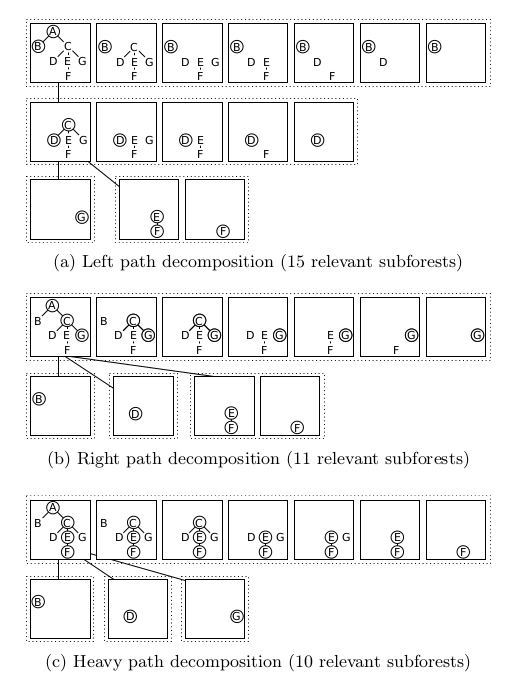
\includegraphics[width=85mm, height=100mm]{../img/LRH_decomposition.png}
%TODO vlastne obrazky
\caption{Celkova dekompozicia pomocou LRH strategii}
\label{obr:LRH_decomposition}
\end{figure}

\begin{definice}
	Relevant subtrees stromu $F$ pre root-leaf cestu $\gamma$ su definovane ako $F - \gamma$.
	Relevant subforests stromu $F$ pre nejaku root-leaf cestu $\gamma$ su definovane rekurzivne ako
	\begin{align*}
    \mathcal{F}(\emptyset, \gamma) &= \emptyset
		\\
		\mathcal{F}(F, \gamma) &= \{F\} \cup
		\begin{cases}
      \mathcal{F}(F - r_{R}(F), \gamma), \quad{} &\text{ak $r_{L}(F) \in \gamma$}
			\\
      \mathcal{F}(F - r_{L}(F), \gamma), &\text{v ostatnych pripadoch}
		\end{cases}
	\end{align*}
\end{definice}

Kazdy krok rekurzie \ref{eq:ted} je vypocitana v konstantnom case z inych podproblemov.
Doba behu zavisi na pocte podproblemov ktore potrebujeme vyratat, takze dekompozicna
strategia hraje velku ulohu v dobe behu algoritmu.

Ulohou RTEDu je najst strategiu s najnizsim poctom problemov, ktore potrebujeme vyratat,
zatial co ulohou GTEDu je podla danej strategie prejst celou rekurziou \ref{eq:ted} a vratit
vzdialenost medzi stromami $F$ a $G$.







